\documentclass[12pt]{article}

%\usepackage{graphics}
\usepackage{graphicx}
\usepackage{caption}
\usepackage{subcaption}
%\usepackage{epsfig}
%\usepackage{times}
%\usepackage{amsmath}
%\usepackage[spanish]{babel}
%\usepackage{lscape}
%\usepackage[nottoc,numbib]{tocbibind}
%\usepackage{pdfpages}

\title{Exercise 1}
\date{\today}
%\author{Mat\'{\i}as Rivero}

\begin{document}
\maketitle

\section{Assignment}
In engineering, the stresses are one of the prinicipal variables which helps to predict the failure of a mechanical component, defined by a specific shape and material, and subjected to specific boundary conditions. The specific points in a given component where stresses ``concentrates'' and tends to infinity in the continumm, must be avoided. Finite element analysis helps to perform this kind of analysis and helps the engineer during the designign process. As the cost of performing a computer simulation of a given problem is low compared with experiments, the engineer has the oportunity to redisign several times a specific component until all usage requeriments are fullfiled. 

\medskip

Let's consider an L-shaped beam made of aluminium subjected only to Dirichlet boundary conditions. The geometry, material properties and boundary conditions are given by Fig.~\ref{fig:geometry}.
\begin{itemize}
\item Run this problem using Ostero and postprocess the results with ParaView. 
\item Look for the point of maximum $\sigma_{xx}$ stress.
\item Refine the mesh and see how this value (and position) evolves. What's happening?
\item Propose a new design to improve this undesired performance.
\item Generate the mesh of your proposed design and perform a mesh convergence analysis to check the improvement.
\end{itemize}

If you get lost, in the RESOLUTION folder you will find several hints that will help you with the fullfilment of this assignment.

\begin{figure}[htp]
\begin{center}
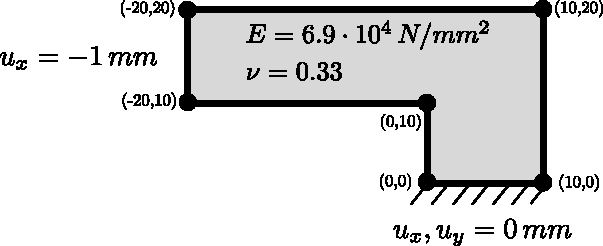
\includegraphics[width=1\linewidth]{Lbeam.pdf}
\caption{Geometry, properties and boundary conditions.}
\label{fig:geometry}
\end{center}
\end{figure}

%~\cite{bib:belytschko}.
%\begin{thebibliography}{9}
%\bibitem{bib:belytschko} {\it Nonlinear Finite Elements for Continua and Structures}. Ted Belytschko, Wing Kam Liu, Brian Moran. Wiley, 2000. 
%\end{thebibliography}

\end{document}
